\section{Diagrama de Conexión}

\subsection{Esquemático del Circuito}
El conexionado físico del sistema optimiza el uso de terminales utilizando un bus I²C compartido y una salida digital para el actuador, como se muestra en la Figura~\ref{fig:diagrama_conexiones}.

\begin{figure}[H]
    \centering
    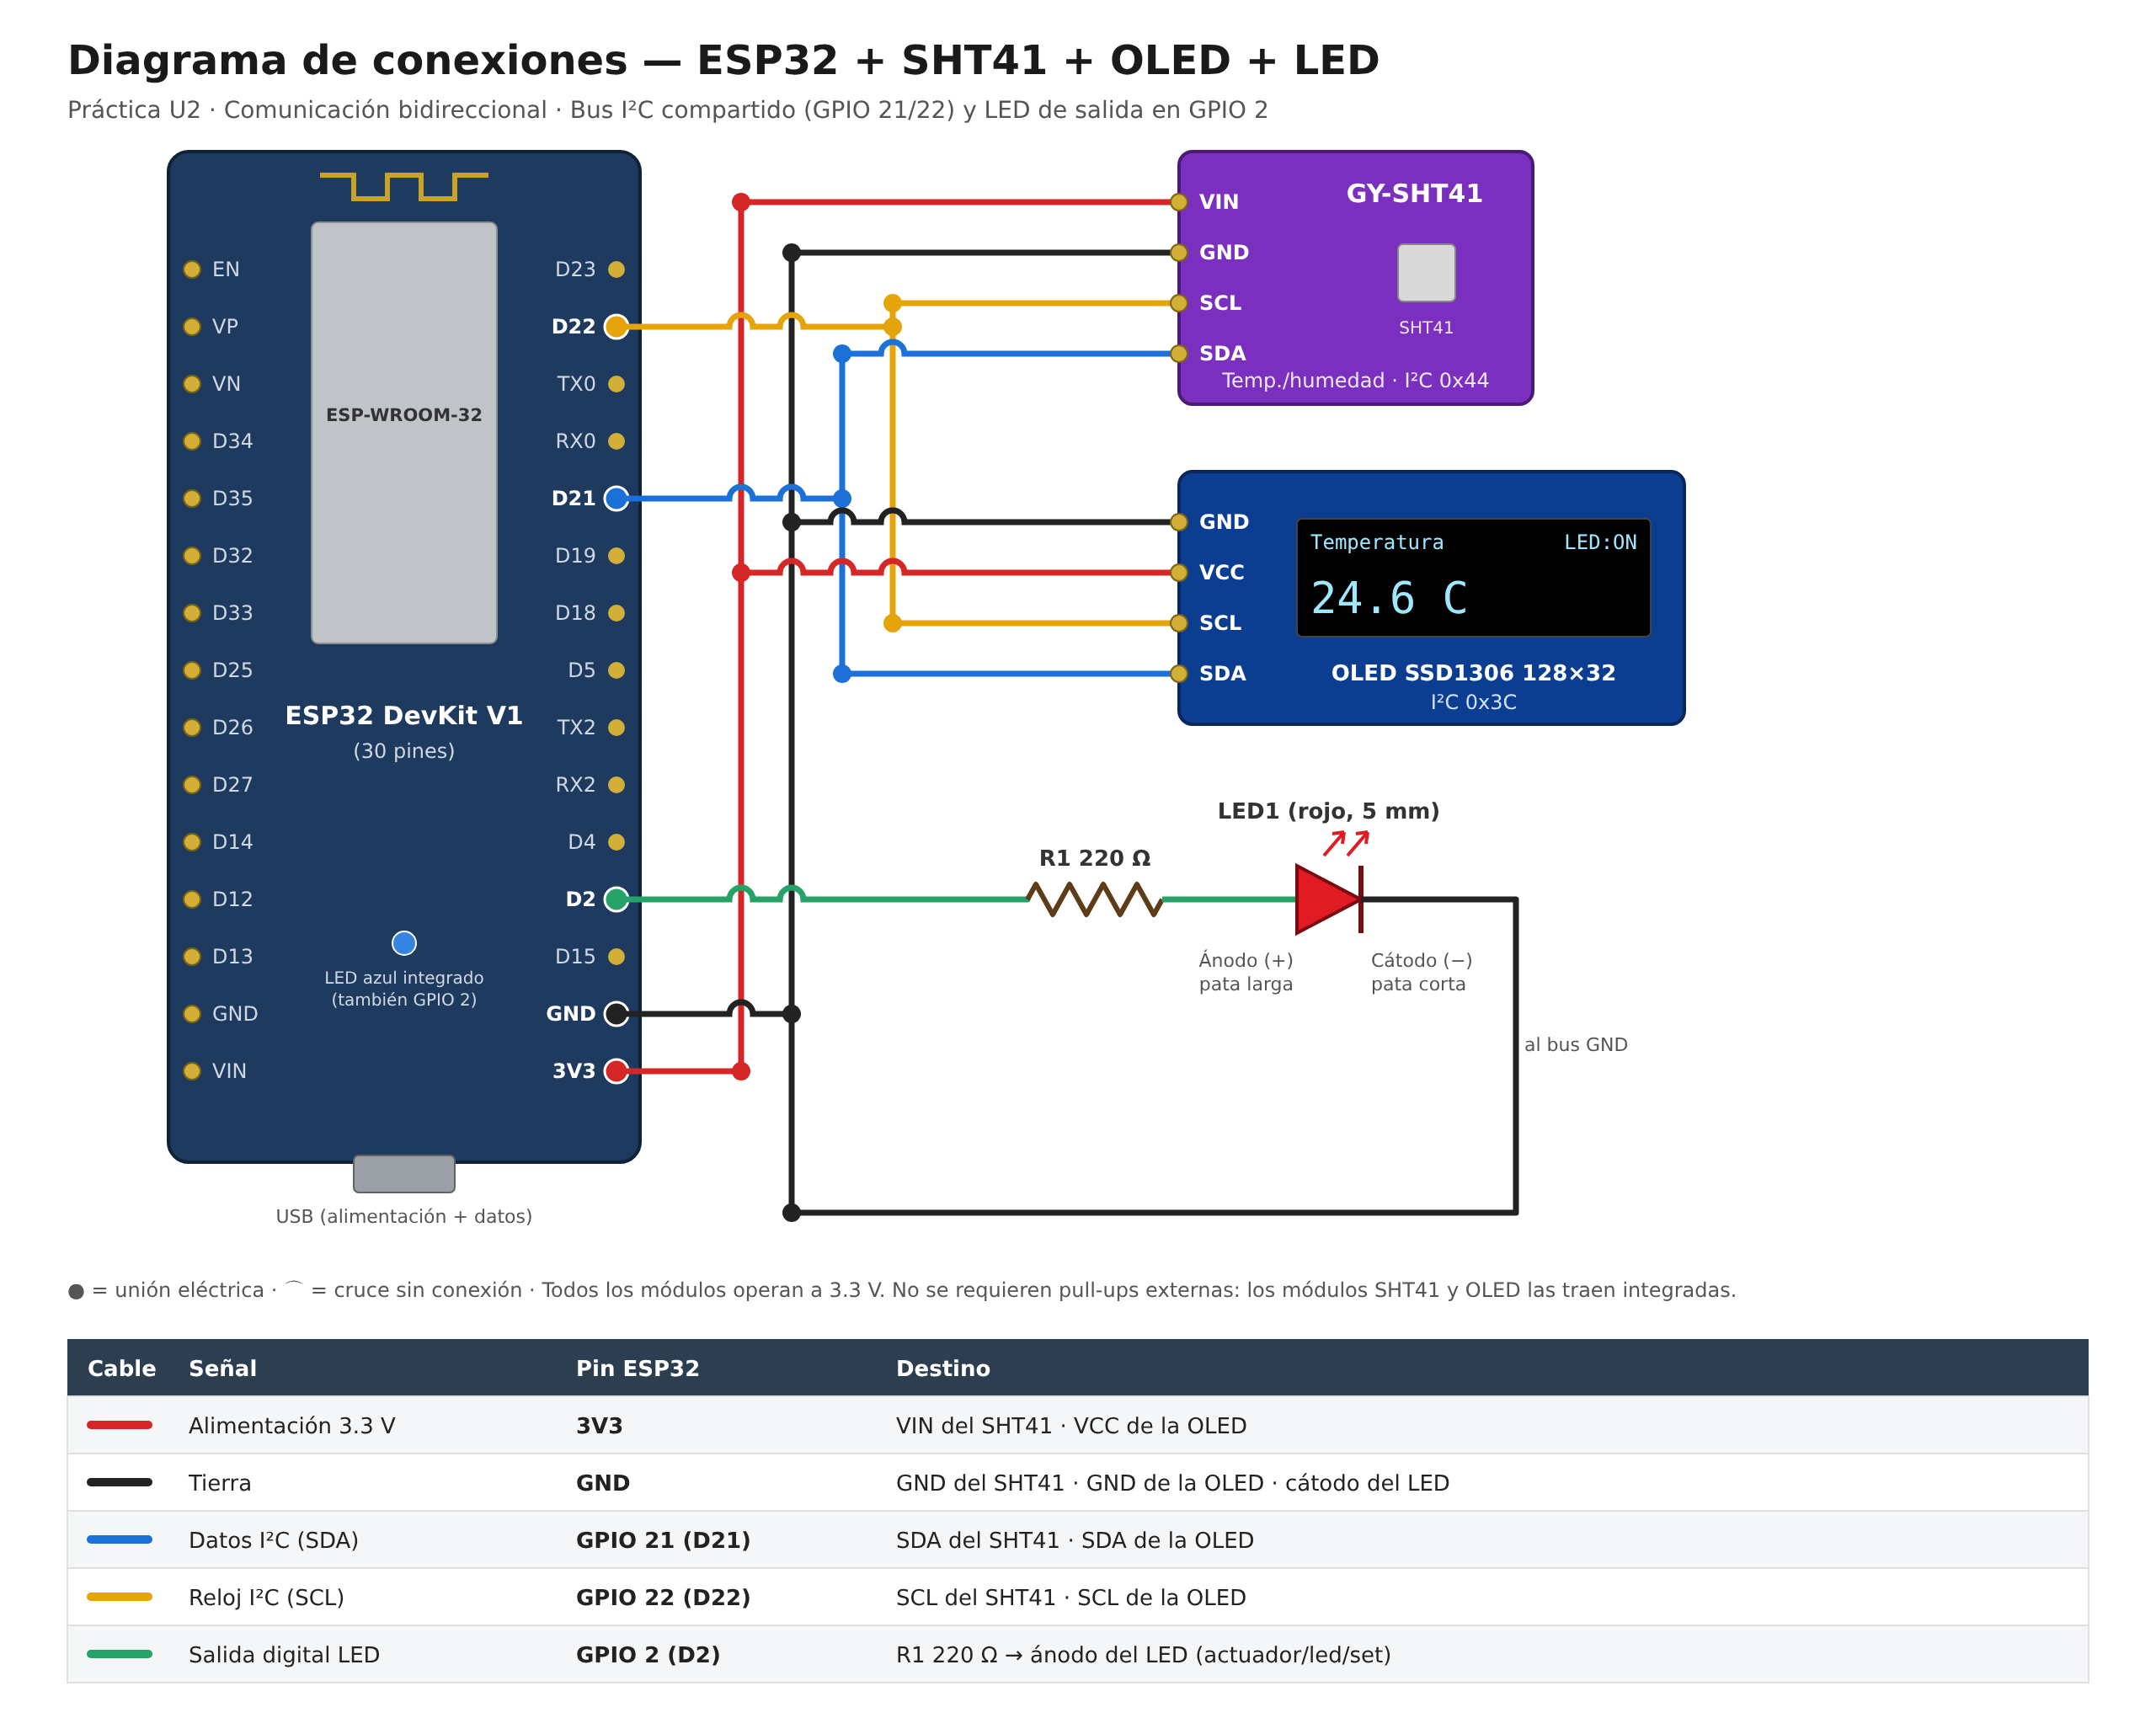
\includegraphics[width=0.92\textwidth]{imagenes/diagrama_conexiones.png}
    \caption{Diagrama de conexión: ESP32 DevKit V1, sensor ambiental SHT41, pantalla OLED y LED en GPIO 2.}
    \label{fig:diagrama_conexiones}
\end{figure}

\subsection{Asignación de Terminales y Conexiones}
\begin{table}[H]
\centering
\small
\begin{tabularx}{\textwidth}{l c l X}
\toprule
\textbf{Señal} & \textbf{Pin ESP32} & \textbf{Destino Físico} & \textbf{Categoría / Propósito} \\
\midrule
\texttt{3V3} & 3V3 & \texttt{VIN} de SHT41 y \texttt{VCC} de OLED & Alimentación lógica regulada (3.3V). \\
\texttt{GND} & GND & \texttt{GND} de SHT41, OLED y cátodo del LED & Referencia común de tierra. \\
\texttt{GPIO 21} & D21 (SDA) & \texttt{SDA} de SHT41 y \texttt{SDA} de OLED & Línea de datos I²C compartida. \\
\texttt{GPIO 22} & D22 (SCL) & \texttt{SCL} de SHT41 y \texttt{SCL} de OLED & Reloj I²C (100 kHz). \\
\texttt{GPIO 2} & D2 & Resistor $220\,\Omega$ $\to$ ánodo LED & \practicaBadge Salida del actuador conmutable. \\
\bottomrule
\end{tabularx}
\caption{Mapeo de pines del circuito.}
\label{tab:pinout}
\end{table}

\subsection{Cálculo Eléctrico del Circuito del LED}
Para un nivel lógico alto en el ESP32 ($V_{OH} \approx 3.3\,\text{V}$) y una caída de tensión típica del LED rojo ($V_F \approx 2.0\,\text{V}$), la corriente de polarización es:
\begin{equation}
    I_{LED} = \frac{V_{OH} - V_F}{R} = \frac{3.3\,\text{V} - 2.0\,\text{V}}{220\,\Omega} = 5.91\,\text{mA}
\end{equation}
La potencia disipada en el resistor es $P = I_{LED}^2 \cdot R \approx 7.68\,\text{mW}$ (muy inferior a la capacidad nominal de $250\,\text{mW}$). La corriente de $5.91\,\text{mA}$ está dentro del límite seguro del pin del ESP32 ($\le 12\,\text{mA}$).

\paragraph{Nota de diseño (Strapping Pin y LED integrado):} El pin \texttt{GPIO 2} es un pin de configuración de arranque (\textit{boot strapping}); la resistencia a GND mantiene el pin en nivel bajo durante el encendido sin interferir con el arranque ni la programación. Además, \texttt{GPIO 2} conmuta en paralelo el LED azul integrado en la placa DevKit.
